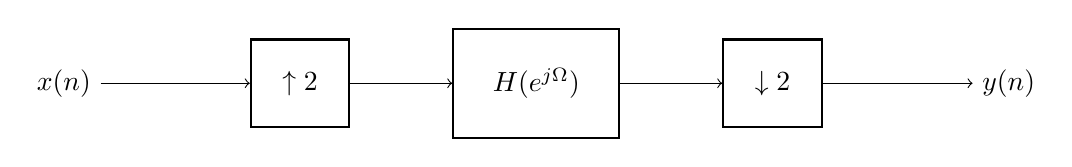
\begin{tikzpicture}
    \node[rectangle,draw,thick,inner sep=0.5cm] (H_W) at (0,0) {$H(e^{j\Omega})$} ;
    \node[xshift=3cm,rectangle,draw,thick,inner sep=0.4cm] (down2) at (H_W) {$\downarrow 2$} ;
    \node[xshift=-3cm,rectangle,draw,thick,inner sep=0.4cm] (up2) at (H_W) {$\uparrow 2$} ;
    \node[xshift=-3cm] (x_n) at (up2) {$x(n)$} ;
    \node[xshift=3cm] (y_n) at (down2) {$y(n)$} ;
    
    % \node[rectangle,minimum width=8cm,minimum height=3cm,dashed,thick,draw] (box) at (H_W) {};
    % \node[yshift=.5cm] (box_label) at (box.north) {$H_{eff}(e^{j\Omega})$};
    
    \draw[->] (x_n) -- (up2) ;
    \draw[->] (up2) -- (H_W) ;
    \draw[->] (H_W) -- (down2) ;
    \draw[->] (down2) -- (y_n) ;
\end{tikzpicture}